\section{Stock Market}

\subsection{Stock Market Fundamentals}
The stock market refers to the collection of markets and exchanges where regular activities of buying, selling and issuance of shares of publicly-held companies take place. It was created a long time ago in order to facilitate the raise of capital of companies, promoting a transparent way of trading regarding company assets. Nowadays, its main purpose is to regulate the exchange of stocks or other financial assets, ensuring a fair environment for both investors and corporations (whose stocks are traded in the market). It can be seen as the staple of the global financial system. The stock market created a dynamic system encouraging permanent innovation and improvement in every domain.

From an investor perspective, each action is the result of an investment strategy which contains a set of rules, behaviours or procedures. Although, there are many investment strategies, most of them can be classified in two separate groups: fundamental analysis and technical analysis. Fundamental analysis represents the analysis of a company's past performance as well as the credibility of its accounts through various factors and indicators based on the financial statements, business trends and general economic conditions. On the other hand, technical analysis is not concerned with any of the company's financial prospects and seeks to determine the future price of a stock based only the trends of the past price (a form of time series analysis). For the following reasons, fundamental analysis is usually seen as a long-term strategy, while technical analysis is seen as a  short-term one.

This thesis will tackle the topic of stock market prediction more from a technical analysis perspective being more suitable for automated non-subjective decisions. We will further evaluate the evolution of different methods and techniques reaching the latest trends of machine learning strategies, more specifically deep learning which at the moment is not well researched for financial time series forecasting research. \cite{sezer2020financial}



\subsection{Techniques in stock market prediction}
Even though the stock market has a long history, only in the last couple of decades we have seen real development and research in terms of techniques to automate or aid the investor in the process of stock market prediction. At our current state, we can group all techniques in the following categories: statistical, pattern recognition, machine learning, sentiment analysis and hybrid.\cite{shah2019stock} At their core, they can be classified as mainly technical analysis, but they can also borrow some aspects from fundamental analysis.

Prior to the emergence of machine learning, statistical techniques were used which they often assumed linearity. However, they were mostly replaced step by step with other techniques which are more and more researched especially with the exponential growth in computational power. All the other categories may be considered to some degree as machine learning, but they are split accordingly due to the fact that they usually have different goals in mind. While pattern recognition works mostly on predicting certain figures or shapes which repeat themselves with unknown periodicity, machine learning category covers many techniques which have some degree of similarity and not being different enough to represent an entire category. Sentiment analysis represents also a trending methodology which have gained a lot of momentum lately even in financial time series analysis, but it is still mostly researched for recommendation systems.

One subcategory of machine learning which haven't been intensively researched due to its only recent success in other domains is represented by deep learning. Deep learning has been a major breakthrough in many domains such as object detection, speech recognition, natural language processing and so on. This thesis will approach the problem of stock market prediction as a time-series problem using the company historic data to predict on a short-term horizon the price or the trend. We will compare the results from both classical perspectives as a regression and as a classification.

\subsection{Difficulties and controversy}
Stock market has been a studied domain for a long time generating debates and controversy regarding whether it is possible or not to consistently predict its movement. The prediction problem is still an open problem due to its complexity taking into account the volatility of the stock market.In the following paragraphs, we will discuss about two theories which have generated controversy among people.

\vspace{5mm}

Chaos theory is a branch of mathematics focusing on the study of chaos - states of dynamical systems whose apparently random states of disorder and irregularities are often governed by deterministic laws that are highly sensitive to initial conditions. One underlying principle of chaos, also called the 'butterfly effect', describes how a small change in one state of a deterministic nonlinear system can result in large differences in a later state. Chaotic behaviour exists and is mostly characterized in natural systems such as weather, climate or even heartbeat irregularities. For this reason, many consider that the weather forecast for example can be considered accurate only in the following 2-3 days.

Coming back to our domain of interest, chaos theory is seen only as a spontaneous occurrence in some systems with artificial components such as the stock market and road traffic. While there exists some research studying the effects of chaos theory in economic and financial systems, the empirical literature that tests for chaos in economics and finance presents very mixed results.\cite{brooks1998chaos} There is little consensus that the chaos theory may only illustrate sudden shocks and crashes of the market which happen very rarely and can be considered insignificant. During the stock market history, there existed unpredictable events called 'black swan' which were characterized by their extreme rarity and severity impact, but no real linkage with the chaos theory has been done.

\vspace{5mm}

The second hypothesis of which we are going to discuss is more closely related to the stock market domain and is called the 'efficient-market hypothesis'. The 'efficient-market hypothesis' is a hypothesis in financial economics that states that asset prices reflect all available information at a given time. This would basically imply that all publicly known information about a company, which obviously includes its price history, would already be reflected in the current price of the stock. Accordingly, changes in the stock price reflect release of new information, changes in the market or random movements around the value that reflects the existing information set. Burton Malkiel, in his influential 1973 work 'A Random Walk Down Wall Street', claimed that stock prices could therefore not be accurately predicted by looking at price history. As a result, Malkiel argued, stock prices are best described by a statistical process called a "random walk" meaning each day's deviations from the central value are random and unpredictable.

However, investors and researchers have disputed the hypothesis both empirically and theoretically. For example, Warren Buffet who is considered by many one of the most successful investors in the world rebutted this hypothesis in its speech in 1984.\cite{businessinsiderwarrenbuffet} Moreover, there are accepted events which are considered 'stock market anomalies' by the hypothesis since they are violations in which consistently abnormal returns could have been earned by some investment strategies that are constructed based on potential market inefficiencies. Not lastly, there are imperfections in the financial markets which are attributed by behavioural economists to a combination of cognitive biases such as overreaction, overconfidence, information bias and many others.


\section{Scientific Problem}
\subsection{Problem definition}
Stock market prediction is the act of trying to determine the future value of a company stock or other financial instrument traded on an exchange. In terms of a general scientific category, the problem will be evaluated from the perspective of a time series. Time series analysis and time series forecasting are the two linked activities which are done over a time series. However, while time series analysis is mostly linked to statistics, time series forecasting has evolved as being mostly referred with machine learning in mind. In comparison with other problems, time series require more attention regarding the processing of data since it has a natural time ordering which must not be broken in any way.

The problem of stock market prediction may also be split depending on what information we want to obtain: regression if we want a continuous output variable such as the closing price of some stock or classification if we only want a hint regarding the future trend. This thesis will try to use both categories for different time horizons such as 1-day, 3-day, 5-day etc. For regression we will have two main versions:
\begin{itemize}
    \item single point in future of the closing price for a company stock
    \item set of points corresponding to each day in the time horizon - allowing us to see the general flow chart of the company stock price
\end{itemize}
For the classification category, we will split it in three or five categories (not decided yet): major decline, minor decline, stagnation, minor increase, major increase. Based on all this variants, we are going to compare and decide how should we interpret all results into an automated algorithm which decides whether to buy or sell.

\subsection{Methodology in training data}
The following subsection will present the details and methodologies behind choosing and preparing the data for future training. As mentioned already in a previous section, stock market prediction may make use of various information in order to attempt forecasting future prices depending on many factors such as the time horizon.

Because we are not going to predict intraday evolution of prices (which is usually done in fast markets as Forex), we are going to use the classic data which is provided for evaluating a company stock value. It is available daily and contains five measurements abbreviated usually as OCHLV:
\begin{enumerate}
    \item Open - the value of a single company stock at the beginning of the daily trading session
    \item Close - the value of a single company stock at the end of the daily trading session
    \item High - the maximum value of a single company stock obtained during the entire daily trading session
    \item Low - the minimum value of a single company stock obtained during the entire daily trading session
    \item Volume - the number of shares that were traded during the entire daily trading session
\end{enumerate}
Based on this data, we could theoretically have a complete technical analysis taking into account only the company's past data. However, we will also add at least one stock market index representative for the market from which the company comes from. Stock market indexes can be seen as powerful indicators for global and country-specific economies. Because we are going to use stock data from popular American companies, we'll choose from S\&P500, DowJonesIndustrial and NasdaqComposite. Using stock market indexes should help the network getting a grip of the general economic trend in addition to only the company's past data which may or may not reflect a lot the past economic trend of the general economy. In terms of actual data that is obtained from these stock market indexes, we are talking about the same five measurements mentioned earlier, but at the level of that stock market index (which is usually seen as a conglomerate of the most important companies of that market). It should be noted that is totally possible to trade only stock market indexes as opposed to trading individual company stocks.

In terms of preprocessing the data, we must standardize in order to aid the model in learning the relevant futures. Due to the fact that we evaluate a time-series problem, a particular attention should be given to the split between training and validation data. Because the validation data is considered to represent the unknown future, the strategy on which we standardize the data must be used only on the training data and applied with the same parameters obtained on the validation data. We are going to experiment with two different methodologies. First, with classic standardization which involves moving each feature values to a mean close to 0 and a standard deviation close to 1. Secondly, we are going to experiment with a min-max scaling which brings a set of values into the interval $[-1, 1]$. It is clear that in both cases, the validation data would not necessary respect the same strict results in the end because the validation data may contain values outside the training data set, but it still is highly important to bring the features much closer since we use data with various interval differences between them.

\subsection{Proposed approach}
Financial time forecasting has been the top problem of computational intelligence for both academic financial researchers and industry investors due to its broad implementation areas and impact. As mentioned previously, many techniques and methodologies have evolved throughout the recent decades alongside the exponential growth in computational power. Machine learning has become one of the headlines in computer science and more recently a sub-domain of machine learning, deep learning, has started to receive the most attention of the industry. Even though deep learning has been recognized as the next breakthrough in many problems such as speech recognition, image recognition, natural language processing and many more, in terms of time series forecasting and more specifically stock market prediction the research is still continuously developing. The current state of art is a lot harder to define since there are many different approaches to what is going to be forecast and how those results should be incorporated in a strategy that would maximize the profit and minimize the loss. Consequently, this thesis will bring a clearer comparison between similar approaches in terms of output results and strategies, but keeping a consistent approach in terms of the actual deep learning model used.

Deep learning at its core is more of an abstract concept representing a class of machine learning that uses multiple layers to progressively extract higher level features from the raw input. In terms of architectures, there are many variants which have seen success in one or more domains: deep neural networks, deep belief networks, recurrent neural networks and convolutional neural networks. For the specific domain of stock market prediction, there has not been decided a definitive architecture which should be seen as the starting stone. However, based on the fact that the problem of stock market prediction can be seen as a time series forecasting problem where the past data should influence the future trend, there is a growing trend in using variations of recurrent neural networks since they were created exhibiting temporal behaviour in mind and some sort of 'memory'. 

\vspace{5mm}

Based on the systematic literature review \cite{sezer2020financial}, we can draw many conclusions from which will orientate our search. We are going to discuss about several topics: subtopics of financial time series prediction considered and categorization of techniques and network structures that were used.

Firstly, let us begin with the subtopics of financial time series which were considered in the literature review. The paper research included not only stock market dependent activities, but also other markets which have a certain connection with it such as commodity (oil, gold etc.), cryptocurrency or forex markets. Even though, there might be certain differences between them, at their core in all applications the same underlying dynamics occur. As mentioned also in this thesis before, all categories can be clustered in two main groups based on their expected outputs price prediction and trend (movement) prediction. Although, price prediction is definitely the harder problem of the two increasing the difficulty exponentially from classification to regression, in terms of financial and economics interests the actual improvements are not seen as a major importance taking into consideration also the risk management. For that main reason, many researchers consider trend prediction a more crucial study area than the actual price prediction considering the actual implications. However, from the statistics of the literature review \cite{sezer2020financial} it can be observed that trend forecasting represent less than 40\% of the actual research considered. Regarding the classification categories which were used two methodologies accounted for almost any study:
\begin{itemize}
    \item two-class approach as in buy or sell which basically represent an upward or downward trend
    \item three-class approach which represent one of the following three patterns: decline, increase or stagnation
\end{itemize}
Other types of classifications are relatively hard to promote or justify for some simple reasons. First, it will be hard to come up with new and justified categories which would not blur the lines between them. Secondly, new categories will imply in theory some percentage margins based on which you would decide for example whether the increase is small or large. Those percentage might also be adjusted depending on how long the time horizon is for the actual predictions. Lastly, more categories would increase the actual difficulty of the problem and can be justified only if you find along a method which would be able to reward the improvements which were attempted. In terms of regression, the main distinctions between solutions without mentioning the time horizon is whether the problem is approached as a single-point or multi-point regression. The difference stems from the actual output of the problem which can be only a single point in the future based on the decided horizon or a set of points for each day in the future until the decided horizon. While the second category is on a whole another level in terms of difficulty, it is also more justified in terms of trying to improve and solve the original classification problem. The first category would eventually be used alongside a investment strategy and a risk management literally in the same way as the classification one, while the actual set of points may offer more hindsight regarding the market future information and changing an actual investment strategy as a whole. In this thesis, we will try compare the results from multiple approaches and attempt to link some of them into an investment strategy algorithm.

\vspace{5mm}

Secondly, we are going to summarize the trending techniques of architectures used in financial time series problems. According to \cite{sezer2020financial} recurrent neural networks dominated in terms of used architectures. The main reason for this occurrence is the actual nature of our problem which implies data across a timeline with time-dependent components. Even though, recurrent neural networks accounted for more than half of the models, we should mention that many variations of recurrent neural networks have been included in this category and classic recurrent neural networks weren't nearly as present as more popular choices (as in other domains) such as long short-term memory (LSTM) or more recently gated recurrent unit (GRU). LSTM networks have been successfully used in domains such as speech recognition, music composition or even time series prediction giving them a stronger sense of security. Besides recurrent neural networks, other techniques were also used such as deep multi layer perceptron (DMLP) due to its acceptance in the past of its 'older brother', the multi layer perceptron (MLP), convolutional neural networks (CNN) or deep reinforcement learning. Taking everything into account, this thesis will use variations composed of LSTM and GRU networks for all the previously mentioned variants of problems due to their recognized worth in another domain and their large flexibility in terms of both classification and regression problems.

\subsection{LSTM and GRU techniques}
In the following subsection, we are going to present the details regarding the structure and characteristics of long short-term memory and gated recurrent unit layers and networks. The discussion will progressively evolve from classic recurrent neural networks to LSTM which were first proposed over two decades ago and finally to GRU which is more of a newer concept being more 'light-weight' than LSTM while maintaining most of their counter-part abilities.

Recurrent neural networks (RNN) have been created with series in mind such that neighbouring inputs might have an influence on each other in some way. A RNN remembers a portion of its past (previous inputs) and influences the results of future inputs. In order to achieve this behaviour, RNN in addition to classic neural networks contain a hidden state which is updated and used for each input received in the series. This hidden state can be thought of as a context based on prior inputs. Moreover, this structure allows to process variable length sequences of inputs, making them applicable for unsegmented tasks such as handwriting recognition. In addition, when speaking of recurrent neural networks we can introduce the topic of 'parameter sharing' which has been successfully used in image classifying convolutional neural networks. However, a major difference should be noted in the actual definition of the neighbour between RNN (elements in a series) and CNN (neighbouring pixels in an image).

Even though, RNN were a significant improvement in the theory of machine learning, their classic versions didn't see much success initially. Practical difficulties have been reported in training recurrent neural networks to perform tasks in which the temporal contingencies present in the input/output sequences span long intervals \cite{bengio1994learning}. Based on the previous citation, it was demonstrated that it exists a trade-off between efficient learning by grading descent and maintaining relevant context information for long periods of time. Practically, RNN usually suffer of the well known problem of 'vanishing gradient'. The main issue arises when training a multi-layer network while using a backpropagation and gradient-based learning algorithms for updating the network values. While the initial error is transmitted along the entire network in order to adjust the weights accordingly, there is an increased chance of getting an update which progressively becomes more and more insignificant for the actual weight of that cell causing a valid update which actually doesn't influence the network behaviour a lot.  Establishing on these aspects, further research was done to search for stricter structures and architectures which would improve the previous state of the art. Long short-term memory has been a major breakthrough in finding structures that would outperform previous networks, being proposed in 1997. As a testimony, even today many applications in different domains representing state of the art are using LSTM architectures under the hood.

Long Short Term Memory networks -abbreviated as LSTM- were introduced by Hochreiter and Schmidhuber in 1997 \cite{hochreiter1997long} and were further refined while replacing classic RNN more and more. The main difference between them is the new structure of a singular cell. While the repeating module between different layers is mostly the same, an LSTM cell has a much more complicated structure in order to address the long-term dependecies issue. In order to compare them and explain the structure we are going to examine and compare two images with the content of each cell.

\begin{figure}[H]

\begin{subfigure}{0.47\textwidth}
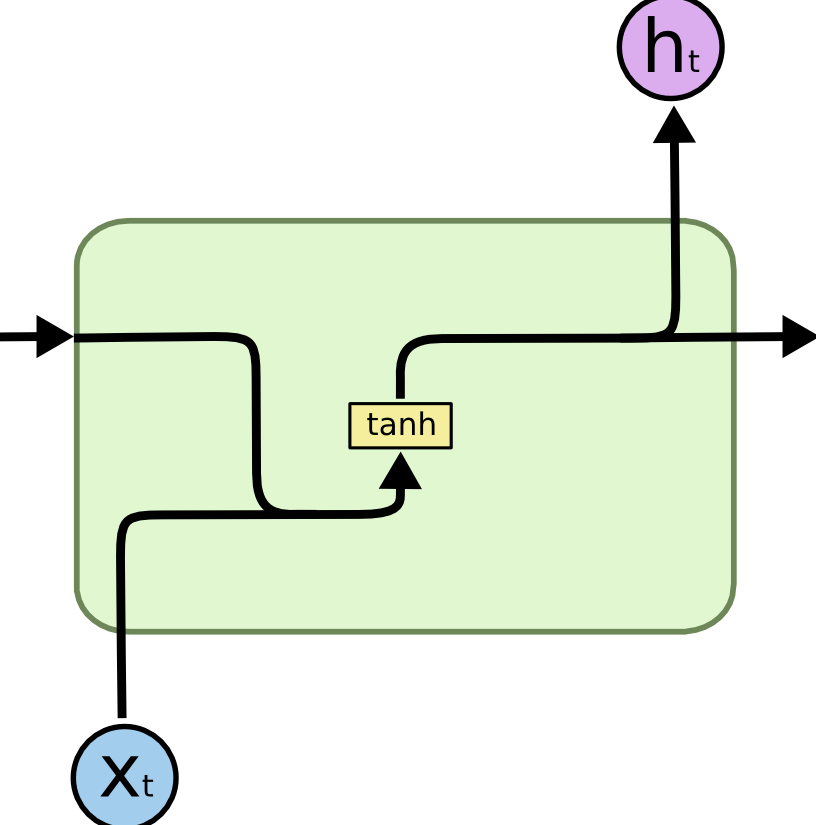
\includegraphics[width=0.9\linewidth, height=5cm]{images/RNNCell.png} 
\caption{Classic Recurrent Neural Network Cell}
\label{fig:rnncell}
\end{subfigure}
\begin{subfigure}{0.47\textwidth}
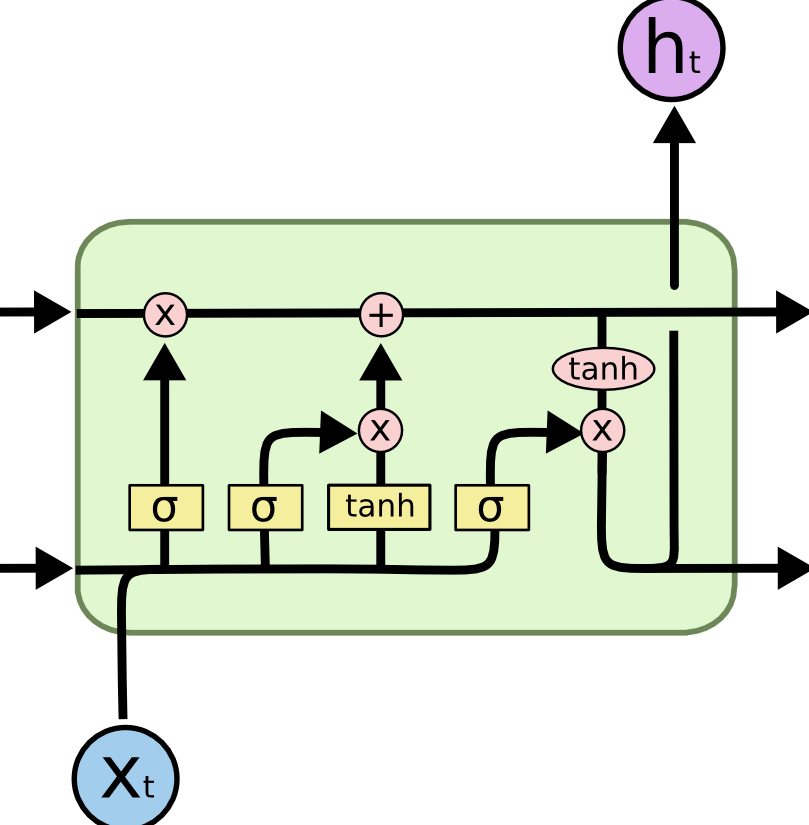
\includegraphics[width=0.9\linewidth, height=5cm]{images/LSTMCell.png}
\caption{Long Short Term Memory Cell}
\label{fig:lstmcell}
\end{subfigure}

\caption{Comparison between Classic Recurrent Neural Network Cell and Long Short Term Memory Cell}
\label{fig:rnnandlstmcomparison}
\end{figure}
\begin{flushright}
Original site: https://colah.github.io/posts/2015-08-Understanding-LSTMs/
\end{flushright}




As we may observe, the LSTM cell maintains the key points of a RNN cell -input vector, tanh to adjust the weights in the interval [-1, 1] and the hidden state- while adding a set of layers inside the cell which create certain structures which are also called gates. Next we are going to create a legend for the elements inside the figure in order to allow us to explain the structure.

\begin{itemize}
    \item $\displaystyle X_t$ - input vector
    \item $\displaystyle h_t$ - hidden state after computation inside the cell
    \item x within a circle - pointwise multiplication
    \item + within a circle - pointwise addition
    \item $\displaystyle \sigma$ - sigmoid function
    \item $\displaystyle tanh$ - hyperbolic tangent function
    \item yellow rectangle - neural network layer
\end{itemize}

Regarding the arrows which enter or exit the figure we have:

\begin{itemize}
    \item first arrow entering (upper half of the figure) - previous cell state denoted $\displaystyle C_{t-1}$
    \item second arrow entering (lower half of the figure) - previous hidden state denoted $\displaystyle h_{t-1}$
    \item first arrow exiting (upper half of the figure) - new computed cell state denoted $\displaystyle C_t$
    \item second arrow exiting (lower half of the figure) - new computed hidden state denoted $\displaystyle h_t$ and also being used as output if necessary
\end{itemize}

The main idea behind LSTMs is the cell state $C_t$ which can be seen more of a consistent value in comparison to the hidden state. From the figure \ref{fig:lstmcell}, the cell state runs along the horizontal line in the upper part. In comparison to the hidden state which suffers many changes and operations, the cell state can be seen as rather regular. This implementation facilitates the flow of past information close to unchanged allowing to maintain long-term dependencies more further in the series. As the cell evolves through the series, information gets added or removed via gates. The gates are small neural networks themselves that decide and learn what information is relevant to keep or forget during training. As mentioned in the previous list, besides pointwise basic operators there are two classic functions applied: tanh and sigmoid. While tanh is used to regulate the network maintaining the values in a small interval [-1, 1], the sigmoid squishes the values between 0 and 1. This approach is useful in easily deciding what to do with the current information. A value close to 0 in a multiplication is equivalent to the idea of forgetting that data, while a value close to 1 represents important data which should be kept as intact as possible.

The interaction between the hidden state, the cell state and the input is dictated in a LSTM cell by some small neural networks called gates. There are three types of gates which we'll further explain: forget gate, input gate and output gate. In order to have a visual perspective, we'll use an edited version of the previous figure for a LSTM cell.

\begin{figure}[H]
\centering
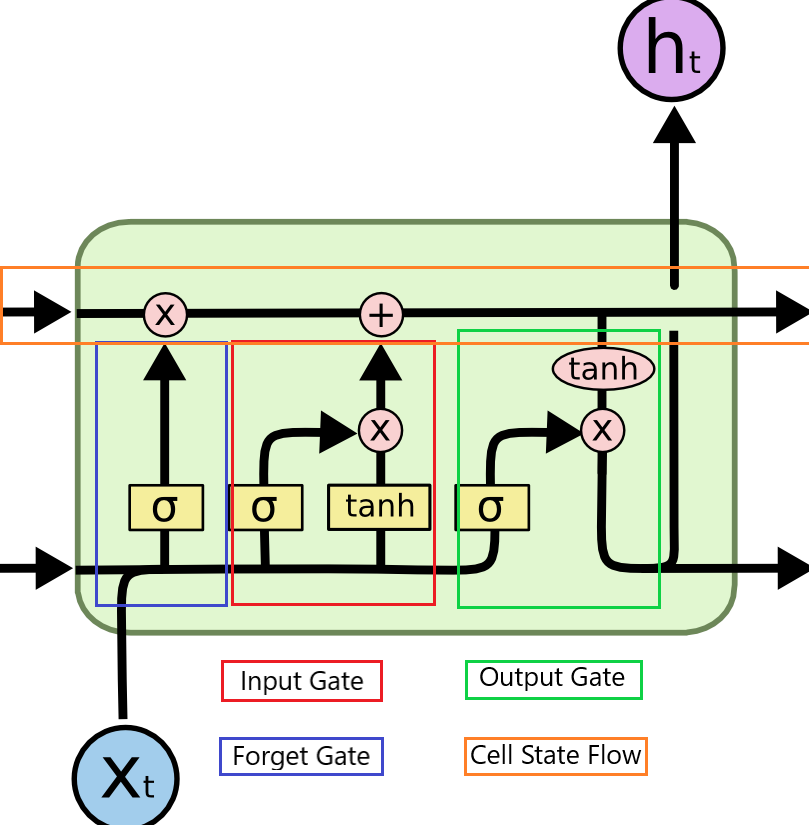
\includegraphics[height=8cm]{images/LSTMCellEdited.png} 
\caption{Edited Long Short Term Memory Cell With Regions}
\label{fig:editedlstmcell}
\end{figure}
\begin{flushright}
Original picture (edited after): https://colah.github.io/posts/2015-08-Understanding-LSTMs/
\end{flushright}

\newpage

\paragraph{Forget Gate}\mbox{} 

\vspace{5mm}

First gate in the flow of a LSTM cell is the forget gate. This layer decides what information is kept and what information is thrown away. As input information for this layer, we use the input vector $\displaystyle x_t$ and the previous hidden state $\displaystyle h_{t-1}$. That information is passed through the sigmoid function which as discussed manages with numbers between 0 and 1 what to forger or remember. The output of this layer is a vector which is used for the previous cell state $\displaystyle C_{t-1}$, consequently having a length equal to that state. If we denote by $\displaystyle f_t$ the output of the forget gate, the following equation may be seen as the behaviour of this layer:
\[ f_t = \sigma(W_f\cdot[h_{t-1}, x_t] + b_f) \]

\paragraph{Input Gate}\mbox{} 

\vspace{5mm}

Second gate in the flow of a LSTM cell is the input gate. The purpose of this layer is to update the content of the cell state based on the new input received. As opposed to the previous layer, this structural gate has a more complicated flow because it must maintain a consistent regulation of the values in the network. The same input as from before, $\displaystyle x_t$ and $\displaystyle h_{t-1}$ is passed on each input branch function: $\displaystyle \sigma$ or $\displaystyle \tanh$. The sigmoid branch is dealing as before of filtering the useful information to be stored later denoted $\displaystyle i_t$, while the tanh branch helps in regulating the network by creating a vector of new candidate values denoted $\displaystyle \Tilde{C}_t$. Combining those two together will obtain the output vector of this gate which will dictate modifications for the new cell state. Let us observe the equations for each branch, while the output vector will be denoted further just by the product of those two:
\[ i_t = \sigma(W_i\cdot[h_{t-1}, x_t] + b_i)\]
\[ \Tilde{C}_t = \tanh(W_C\cdot[h_{t-1}, x_t] + b_C)\]

\paragraph{Cell State Updates}\mbox{} 

\vspace{5mm}

Before moving on to the last gate of a LSTM cell, there must be a discussion first about the update of the cell state which has already received two vectors from the previous gates. The cell state flow begins with the previous values denoted $\displaystyle C_{t-1}$ which are pointwise multiplied with $\displaystyle f_t$, the output vector of the forget gate. The result of this first set of operations is further advanced in the flow in order to incorporate the new result of the next set of layers, the input gate output vector denoted $\displaystyle i_t * \Tilde{C}_t$. In terms of mathematical operations, the output vector is simple pointwise added to the previous result obtained in the flow. After this step, the value obtained is the final cell state for this iteration and will be lastly used in the computations of the new hidden state. The mathematical equation of computing the cell state with mentioned notations is:
\[ C_t = C_{t-1} * f_t + i_t * \Tilde{C}_t\]

\paragraph{Output Gate}\mbox{} 

\vspace{5mm}

The last set of operations in a LSTM cell are represented by the output gate. Its purpose is to decide the content of the next hidden state based on all previous information and operations. From figure \ref{fig:editedlstmcell}, we can observe that we are going to unify the previous hidden state, the input vector and the newly computed cell state. The sigmoid layer as before decides which parts are going to be relevant, in this case which parts are going to be relevant to output. The sigmoid result will be denoted as $\displaystyle o_t$ to represent the output vector. The newly computed cell state is passed through a tanh function which regulates the values for the new hidden state. The results are multiplied pointwise obtaining the new hidden state which is the output for our gate and is also represented as the output in prediction problems. The equivalent mathematical operations are:
\[ o_t = \sigma(W_o\cdot[h_{t-1},x_t]+b_o)\]
\[ h_t = o_t * \tanh(C_t) \]

In order to offer a different perspective for the whole theory behind a LSTM cell, a pseudo-Python code will be attached to represent all discussed operations.

\begin{algorithm}
\caption{Pseudo-Python code for the flow of one LSTM cell}
\label{lstmcellpseudocode}
\lstinputlisting[language=Python]{algorithms/lstmcell.py}
\end{algorithm}

Finally, we are going to talk about Gated Recurrent Unit (GRU) neural network layer. It was introduced recently, in 2014. GRU has many similarities with LSTM as the existence of a forget gate, but has fewer parameters allowing the overall network structure to become more 'lightweight' and reducing training times. In terms of performance, there have been different studies reigning in favor of one or another, but in most types of problems they perform similarly in terms of accuracy and the choice is at the latitude of the developer. As with the LSTM, we will attach a picture regarding the structure of one cell and comparing it.

\begin{figure}[H]
\centering
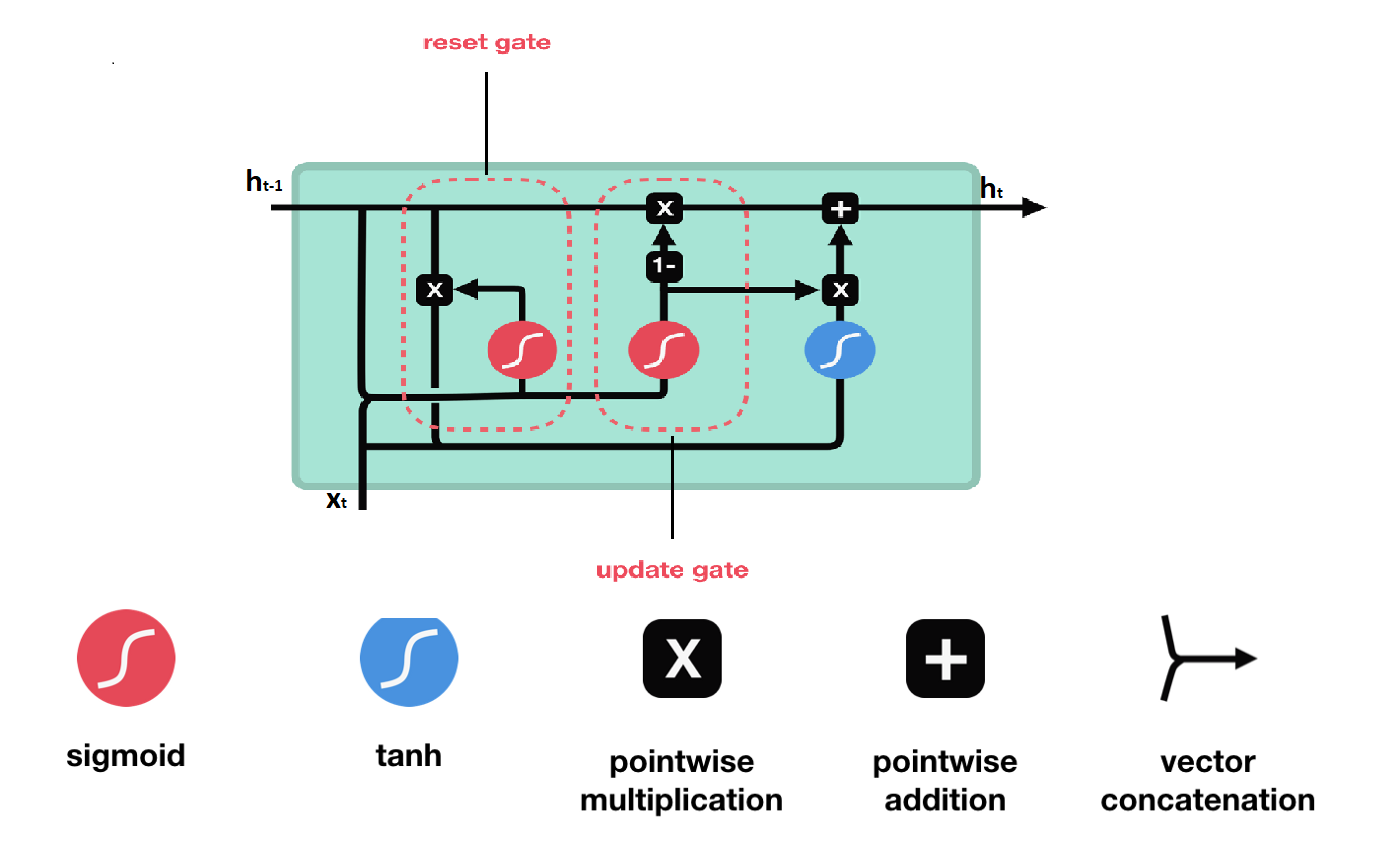
\includegraphics[height=8cm]{images/GRUCell.png} 
\caption{Gated Recurrent Unit Cell}
\label{fig:grucell}
\end{figure}
\begin{flushright}
Original picture (edited after): https://towardsdatascience.com/illustrated-guide-to-lstms-and-gru-s-a-step-by-step-explanation-44e9eb85bf21
\end{flushright}


As before we can observe the same main operators: sigmoid function, hyperbolic tangent function, pointwise addition or multiplication. However, we can clearly see a reduction in the number of gates and consequently operations.

\paragraph{Reset Gate}\mbox{}

The reset gate decides the amount of past information to forget by using both the previous hidden state of the cell $\displaystyle h_{t-1}$ and the current input vector $\displaystyle x_t$. While at the first glance it may seem similar to the forget gate from an LSTM, in reality they serve different purposes. We are going to denote with $\displaystyle r_t$ the result of this gate operation which we'll be used further.
\[ r_t = \sigma(W_r\cdot[h_{t-1}, x_t])\]


\paragraph{Update Gate}\mbox{}

The update gate represents a clear distinction from LSTM by creating from two different gates, forget and input, a single gate in GRU. It decides what information is added and what information is thrown away respectively. We'll denote by $\displaystyle z_t$ the first result of the sigmoid in the update gate which is passed in two separate sets of operations which will finally construct the new hidden state $\displaystyle h_t$.
\[ z_t = \sigma(W_z\cdot[h_{t-1}, x_t])\]

GRU doesn't have anymore an output gate since the cell state and the hidden state are merged at the end. On the last set of operations will denote with $\displaystyle \Tilde{h}_t$ the result representing the current memory content which in the end is linked with the results from the update gate to compute the final hidden state $\displaystyle h_t$.
\[ \Tilde{h}_t = \tanh(W\cdot [r_t * h_{t-1}, x_t]) \]
\[ h_t = (1 - z_t) * h_{t-1} + z_t * \Tilde{h}_t\]

Finally, before moving to the next subsection we are going to address two studies regarding the general performance and structure of the LSTM and its counterparts. While the discovery of the LSTM structure may seem at first to some small degree random, since then many studies were done in order to find an improve architecture which is able to constantly outperform the classic one.

Firstly, we are going to cite "An Empirical Exploration of Recurrent Network Architectures" \cite{jozefowicz2015empirical} which is a study conducted in 2015 for searching various architectures starting from LSTM. The methodology was empirical consisting in algorithm very similar to Genetic Programming. A set of best architectures is at each step maintained and mutations are conducted in order to search for new solutions. Each architecture was filtered initially with a classic memorization problem and after a set of more 'real-life' simulation problems were conducted to address an accuracy. They have gone through over ten thousands architectures finding that no architecture consistently beat LSTM and GRU on the whole set of problems considered. An important remark found is that the LSTM network must contain a bias of 1 to the forget gate in order to be able to maintain a high performance (mentioned in the initial LSTM paper, but forgotten often).

The other citation used is "LSTM: A Search Space Odyssey" \cite{greff2016lstm} which tried to tackle the same problem. However, they only considered nine architectures and evaluated the influence of hyperparameters across a set of problems. In terms of hyperparameters, the learning rate and hidden layer size influence the performance the most, while other hyperparameters such as input noise were found to diminish the results for most architectures. In the end, they concluded that some elements of the LSTM can be eliminated or merge in order to gain training time improvements, but the overall performance of the architectures is very similar across the tested problems with fine-tuned parameters.


\subsection{Results}
